\documentclass[11pt,letterpaper]{article}

\usepackage[margin=0.85in]{geometry}
\usepackage{amsmath,amssymb,amsthm}
\usepackage{booktabs}
\usepackage{array}
\usepackage{xcolor}
\usepackage{tikz}
\usepackage{pgfplots}
\pgfplotsset{compat=1.18}
\usepackage{microtype}
\usepackage{xurl}
\usepackage{hyperref}
\usepackage{enumitem}
\usepackage{fancyhdr}
\usepackage{placeins}
\setlength{\emergencystretch}{1.8em}

\definecolor{plnDark}{HTML}{0B1320}
\definecolor{plnEmerald}{HTML}{059669}
\definecolor{plnCyan}{HTML}{0284C7}
\definecolor{plnGold}{HTML}{D97706}
\definecolor{plnCrimson}{HTML}{DC2626}
\definecolor{plnViolet}{HTML}{7C3AED}

\hypersetup{
  colorlinks=true,
  linkcolor=plnCyan,
  citecolor=plnEmerald,
  urlcolor=plnCyan,
  pdftitle={PLANARIA v2.3.0: Progressive Holographic Executable Architecture (.hbin), Multi-Stratum Compilation, Autonomous Control-Flow Anastomosis, Cryptographic Cellular Quorum, and 6-Kernel Lean 4 Verification},
  pdfauthor={Alexander Stephen Donahue (Independent Researcher, 0thernes project, ORCID 0009-0006-8168-9648)}
}

\pagestyle{fancy}
\setlength{\headheight}{14pt}
\fancyhf{}
\fancyhead[L]{\footnotesize\textsc{PLANARIA v2.3.0 --- Progressive Holographic Executable Architecture}}
\fancyhead[R]{\footnotesize\textsc{Donahue (0thernes)}}
\fancyfoot[C]{\footnotesize\thepage}
\renewcommand{\headrulewidth}{0.4pt}

\newtheorem{theorem}{Theorem}
\newtheorem{proposition}[theorem]{Proposition}
\theoremstyle{remark}
\newtheorem{remark}{Remark}

\title{\vspace{-1.0em}\textbf{PLANARIA v2.3.0: Progressive Holographic Executable Architecture (\texttt{.hbin}), Multi-Stratum Compilation, Autonomous Control-Flow Anastomosis, Cryptographic Cellular Quorum, and 6-Kernel Lean~4 Verification}}

\author{%
  \textbf{Alexander Stephen Donahue}\thanks{%
    ORCID: \href{https://orcid.org/0009-0006-8168-9648}{\texttt{0009-0006-8168-9648}}.
    Affiliation: Independent Researcher (0thernes project), Spokane, WA, USA.
    Email: \href{mailto:0_0@0thernes.art}{\texttt{0\_0@0thernes.art}}.
    Web: \href{https://0thernes.art}{\texttt{https://0thernes.art}}.
    Repository: \href{https://github.com/0thernes/planaria}{\texttt{https://github.com/0thernes/planaria}}.
    Self-funded independent research; governed by the Cosmogonic License (Non-Commercial Research \& Play).
  }\\
  \small Independent Researcher (0thernes project), Spokane, WA, USA
}

\date{November 25, 2026 \quad $\cdot$ \quad Technical Research Preprint \texttt{v2.3.0}}

\begin{document}
\maketitle
\thispagestyle{plain}

\begin{abstract}
Classical compiled executables (\texttt{ELF}, \texttt{PE}, \texttt{Mach-O}, \texttt{WebAssembly}) obey a brittle monolithic topology: corrupting byte~0 of a file header, shifting byte alignment, flipping a single bit in active machine code, or slicing a binary in half induces immediate loader rejection or fatal runtime faults. Wrapping an executable in a conventional flat $(n,k)$ Maximum Distance Separable (MDS) erasure code eliminates localized fragility above $k/n$ survival, yet creates an abrupt \emph{all-or-nothing erasure cliff}---100\% recovery at $k$ surviving shards and 0\% execution at $k-1$---while exposing finite-field Gaussian elimination to catastrophic single-cell Byzantine decoder poisoning.

We present \textbf{PLANARIA v2.3.0}, a complete, zero-dependency, adversarially hardened systems architecture realizing \emph{Progressive Holographic Instruction Stratification (PHIS)}. PLANARIA integrates: (1)~a headerless, byte-granular self-synchronizing 512-byte cellular executable format (\texttt{.hbin}, 192 cells = 98,304~bytes) combining 2-way interleaved inner $\mathrm{RS}(254,238)$ Berlekamp--Massey/\allowbreak Chien/\allowbreak Forney byte-error correction, Depth-8 domain-separated (\texttt{0x00}/\texttt{0x01}/\texttt{0x02}) SHA-256-128 Merkle cell authentication with Overlap-Eclipse defense and O(1) sync-flood bypass, and outer Cauchy-matrix MDS erasure coding over $\mathrm{GF}(2^8)$ (\texttt{0x11D}); (2)~a structured multi-stratum systems language and compiler (\texttt{Plang}) with bounded AST depth, prototype-safe symbol tables, register-windowed function calls, and scratch-register overflow guards; (3)~a sandboxed 32-bit register virtual machine (\texttt{PVM-32}) featuring descending \texttt{ORGAN\_\allowbreak CALL} \emph{Control-Flow Anastomosis} and an ABI-verified, live-host, sovereignty-enforced \emph{Cross-Species Executable Xenograft} splicer; (4)~a WebGL2 3D temporal-quantum Studio driven live by four compiled \texttt{.hbin} species; and (5)~\textbf{70 pure Lean~4 (\texttt{v4.35.0}, \texttt{module} system, zero Mathlib) machine-checked theorems} with zero \texttt{sorryAx}, zero \texttt{native\_\allowbreak decide}, and zero custom axioms, exported as standalone Palomar \texttt{Challenge.lean}/\allowbreak\texttt{Solution.lean} specifications checked across \textbf{6 independent kernels}.

Pre-registered paired empirical benchmarks (\textbf{28/28} verification, property-based, metamorphic, CLI, and HTTP security suites; \textbf{10/10 = 100.0\%} surgical mutants killed) confirm: zero-overlap unaligned 50/50 \emph{Planarian Binary Mitosis} across 6 exact and prime offsets (100\% SHA-256 bit-exact dual regeneration in \textbf{12.57--14.21~ms}); statistically decisive survival past the 75\% cliff of an \textbf{equal-storage flat $\mathrm{RS}(192,48)$ control}---\textbf{100.0\%} at 76\% erasure ($p_{\text{Holm}}=4.55\times 10^{-11}$, Cohen's $h=3.142$), \textbf{95.0\%} at 80\% ($p_{\text{Holm}}=1.75\times 10^{-10}$, $h=2.691$), \textbf{82.5\%} at 88\% ($p_{\text{Holm}}=5.12\times 10^{-9}$, $h=2.278$), and \textbf{65.0\%} at 92\% ($p_{\text{Holm}}=6.26\times 10^{-7}$, $h=1.875$) versus \textbf{0.0\%} for monolithic \texttt{LINBIN01}, $\mathrm{RS}(40,16)$, and equal-storage $\mathrm{RS}(192,48)$; \textbf{100.0\% healing of simultaneous 16-byte contiguous burst errors inside all 192 cells} (3,072 corrupted bytes, 3.13\%) with 0\% survival and 0 silent miscorrections at 18~B; \textbf{100.0\% quarantine of 1--192 RS-valid Byzantine Trojans}; \textbf{5/5 trap-free Cross-Species Xenograft Chimeras}; and \textbf{5.994~ms} median decode (IQR 0.268~ms) with \textbf{42.85~MIPS} (\texttt{0.041~ms/frame} median) \texttt{PVM-32} execution.
\end{abstract}

\noindent\textbf{Keywords:} holographic executables, progressive erasure coding, Cauchy MDS, Reed--Solomon, Merkle trees, Byzantine fault tolerance, virtual machines, graceful degradation, Lean~4 multi-kernel verification.

\section{Introduction, Problem Formulation, and Claims Ledger}
\label{sec:intro}

Compiled binary containers (\texttt{ELF}, \texttt{PE}, \texttt{Mach-O}, \texttt{WebAssembly}) assume reliable contiguous byte-addressed storage where a header at offset~0 maps linear segments (\texttt{.text}, \texttt{.rodata}, \texttt{.data}). Under physical decay, truncation, unaligned streaming, or adversarial injection, this layout exhibits four coupled pathologies:
\begin{enumerate}[leftmargin=1.8em, itemsep=1.5pt]
  \item \textbf{Header Single Point of Failure:} Destroying bytes \texttt{0..63} or prepending 1~byte of unaligned noise causes immediate loader rejection despite 99.9\% intact machine instructions.
  \item \textbf{Single-Rate Erasure Cliff:} Wrapping a binary in a flat $(n,k)$ Reed--Solomon code \cite{reed1960} eliminates localized fragility above $k/n$ survival, yet produces an all-or-nothing discontinuity: at $k-1$ shards, availability drops instantaneously from 100\% to 0\%.
  \item \textbf{Byzantine Poisoning Amplification:} Solving $D = M^{-1} P$ over $\mathrm{GF}(2^8)$ mixes every input shard linearly across every output block; injecting even one RS-valid forged shard with a colliding coordinate corrupts nearly the entire decoded kernel.
  \item \textbf{Rigid Organ Coupling:} Classical executables cannot amputate a damaged graphics or audio organ at runtime, reroute control flow onto a surviving low-resolution stem fallback without halting, or splice ABI-compatible organs across distinct species at raw byte level.
\end{enumerate}

Drawing structural inspiration from planarian regeneration \cite{reddien2004}---strictly as an engineering metaphor, not a biological claim---and grounded mathematically in Priority Encoding Transmission \cite{albanese1996}, rateless codes \cite{luby2002}, Cauchy MDS matrices \cite{bloemer1995,plank2006}, algebraic Reed--Solomon decoding \cite{berlekamp1968,massey1969,chien1964,forney1965,singleton1964}, Barker synchronization \cite{barker1953}, and Merkle authentication trees \cite{merkle1987}, \textbf{PLANARIA v2.3.0} resolves all four pathologies inside a single, auditable, zero-dependency stack. To enforce strict epistemic discipline, Table~\ref{tab:claims} enumerates every primary claim alongside its verification artifact and falsification boundary (mirrors \texttt{CLAIMS.md}).

\begin{table}[ht]
\centering
\caption{PLANARIA v2.3.0 Numbered Claims Ledger, Verification Evidence, and Explicit Falsification Criteria.}
\label{tab:claims}
\footnotesize
\setlength{\tabcolsep}{4pt}
\begin{tabular}{@{} c >{\raggedright\arraybackslash}p{4.3cm} >{\raggedright\arraybackslash}p{4.5cm} >{\raggedright\arraybackslash}p{5.5cm} @{}}
\toprule
\textbf{ID} & \textbf{Claim} & \textbf{Verification Authority} & \textbf{Explicit Falsification Condition} \\
\midrule
\textbf{C1} & $\mathrm{GF}(2^8)$ (\texttt{0x11D}) field laws \& universal 2$\times$2 Cauchy lossless decode & Lean~4 \texttt{GF256.lean} (16 thms, 6 kernels) + \texttt{Suite 01, 25, 27} & Any pair/triple violating field laws or $k$ distinct shards failing Gauss--Jordan inversion \\
\textbf{C2} & Zero-overlap 50/50 unaligned mitosis (exact \& prime offsets) & Lean~4 \texttt{MitosisBounds.lean} (12 thms) + \texttt{Suite 04, 16, 22} & Any aligned or prime half-cut failing bit-exact SHA-256 dual regeneration \\
\textbf{C3} & Zero-cliff progressive bootability beyond flat $\mathrm{RS}(192,48)$ 75\% cliff & Lean~4 \texttt{StratumAnastomosis.lean} (7 thms) + \texttt{benchmarks.json} & Survival failing to beat equal-storage $\mathrm{RS}(192,48)$ at 76--92\% ($p_{\text{Holm}} \ge 0.01$) \\
\textbf{C4} & Tight 16~B/cell simultaneous burst repair \& 17--18~B sharp rejection & Lean~4 \texttt{ByzantineImmune.lean} + \texttt{Suite 02, 07} + \texttt{M04} & Any $\le 16$~B/cell burst failing repair or any $\ge 18$~B burst silently miscorrecting \\
\textbf{C5} & 0\% Byzantine poisoning under pinned Merkle quarantine & Lean~4 \texttt{ByzantineImmune.lean} + \texttt{Suite 08, 12} + \texttt{M01} & Any forged RS-valid cell entering Cauchy inversion under pinned lineage root \\
\textbf{C6} & Sovereign B0/B6 xenograft safety, \texttt{BitVec 32} RAM $<4096$, 0-trap chimeras & Lean~4 \texttt{XenograftABI.lean} (7 thms) + \texttt{Suite 10, 20, 26} + \texttt{M02, M07} & Any graft mutating B0/B6, grafting onto dead host, escaping RAM, or trapping \\
\textbf{C7} & 4-qubit gate unitarity, Horodecki CHSH ($2\sqrt{2}$), Mermin ($|M_4|$), 360-f rewind & Lean~4 \texttt{QuantumTemporal.lean} (12 thms) + Suites 13--15, 25--27 & Norm drift $>10^{-12}$, local-unitary CHSH drift, or rewind state/skill-point leak \\
\textbf{C8} & Hardened compiler, CLI, HTTP CSP/traversal defense \& 10/10 mutation kill & Suites 18--28 + \texttt{scripts/mutation-test.mjs} (10/10 killed) & Any surviving mutant, syntax/sink lint hit, traversal/XSS bypass, or stale artifact \\
\bottomrule
\end{tabular}
\end{table}

\section{Threat Model and Operational Guarantees}
\label{sec:goals}

PLANARIA enforces five simultaneous properties over untrusted raw byte streams (full STRIDE analysis in \texttt{docs/threat-model.md}):
\begin{itemize}[leftmargin=1.6em, itemsep=1.5pt]
  \item \textbf{G1 (Zero-Header Framing, Backward Flywheel \& DoS Defense):} Harvest cells via a byte-granular sliding-window correlator with iterative backward flywheel (recovering preceding cells even if cell~0's 4~B sync marker is obliterated), O(1) \texttt{PLN\textbackslash xB7} sync-flood bypass, and explicit DoS scan caps (\texttt{maxInputBytes}, \texttt{maxSyncCandidates}, \texttt{maxRsFailures}).
  \item \textbf{G2 (Zero-Overlap Unaligned Mitosis):} Any 50/50 physical bisection (exact or prime offset) allows both disjoint halves to boot at Stratum~3 and regenerate a 100\% SHA-256 bit-exact replica.
  \item \textbf{G3 (Zero-Cliff Progressive Execution):} Degrade monotonically across four capability strata ($\mathrm{S3}\to\mathrm{S2}\to\mathrm{S1}\to\mathrm{S0}$ Ghost) down to 4--24\% survival without unhandled VM traps, strictly outperforming both single-stratum $\mathrm{RS}(40,16)$ and equal-storage flat $\mathrm{RS}(192,48)$ past the 75\% erasure cliff.
  \item \textbf{G4 (Dual-Layer ECC \& Byzantine Quarantine):} Heal up to 16 contiguous burst bytes inside \emph{every} 512-byte cell simultaneously and quarantine 100\% of RS-valid forged Byzantine cells prior to Cauchy inversion under a pinned lineage root.
  \item \textbf{G5 (Sovereign Xenograft Splicing \& Runtime Confinement):} Require pinned lineage authority (or explicit \texttt{--allow-unpinned-xenograft} opt-in), require a living host (\texttt{bundles[0].viable}), block Kernel/Genome (\texttt{B0}/\texttt{B6}) replacement even under forged header flags, isolate \texttt{PVM-32} RAM via \texttt{\& 0xFFF}, and bound execution fuel.
\end{itemize}

We assume a computationally bounded adversary who knows the complete \texttt{.hbin} format, constructs zero-syndrome interleaved $\mathrm{RS}(254,238)$ parity, and injects Overlap-Eclipse sync decoys or forged cells ahead of authentic shards, but cannot invert domain-separated FIPS~180-4 SHA-256 \cite{fips180} truncated to 128~bits ($2^{128}$ second-preimage resistance). In \emph{Unpinned Quorum Mode}, an adversary controlling $>50\%$ of surviving RS-valid cells can win cluster election; we prove this exact boundary in Lean~4 (\texttt{unpinned\_quorum\_sybil\_counterexample}) and require pinned roots for adversarial deployments.

\section{The \texorpdfstring{\texttt{.hbin}}{.hbin} v1.0 Cellular Holographic Binary Specification}
\label{sec:hbin}

A pristine \texttt{.hbin} executable is exactly \textbf{98,304 bytes (96~KiB)}, composed of \textbf{192 fixed 512-byte Holographic Cells} with no file header, footer, or central table, framed by a fuzzy ($\le 3$-bit Hamming tolerance) 32-bit sync marker \cite{barker1953}. Figure~\ref{fig:cell} shows the byte-exact 512-byte envelope.

\begin{figure}[ht]
\centering
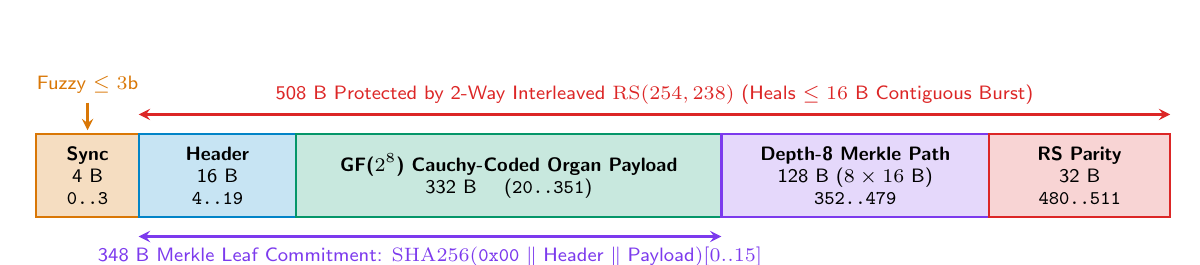
\begin{tikzpicture}[font=\scriptsize\sffamily, >=stealth]
  \fill[plnGold!25, draw=plnGold, thick] (0,0) rectangle (1.3,1.05);
  \node[align=center] at (0.65,0.52) {\textbf{Sync}\\4 B\\\texttt{0..3}};

  \fill[plnCyan!22, draw=plnCyan, thick] (1.3,0) rectangle (3.3,1.05);
  \node[align=center] at (2.3,0.52) {\textbf{Header}\\16 B\\\texttt{4..19}};

  \fill[plnEmerald!22, draw=plnEmerald, thick] (3.3,0) rectangle (8.7,1.05);
  \node[align=center] at (6.0,0.52) {\textbf{GF($2^8$) Cauchy-Coded Organ Payload}\\332 B \quad (\texttt{20..351})};

  \fill[plnViolet!20, draw=plnViolet, thick] (8.7,0) rectangle (12.1,1.05);
  \node[align=center] at (10.4,0.52) {\textbf{Depth-8 Merkle Path}\\128 B ($8\times 16$ B)\\\texttt{352..479}};

  \fill[plnCrimson!20, draw=plnCrimson, thick] (12.1,0) rectangle (14.4,1.05);
  \node[align=center] at (13.25,0.52) {\textbf{RS Parity}\\32 B\\\texttt{480..511}};

  \draw[thick, plnViolet, <->] (1.3,-0.25) -- (8.7,-0.25)
    node[midway, below, text=plnViolet] {348 B Merkle Leaf Commitment: $\mathrm{SHA256}(\texttt{0x00}\parallel\text{Header}\parallel\text{Payload})[0..15]$};

  \draw[thick, plnCrimson, <->] (1.3,1.30) -- (14.4,1.30)
    node[midway, above, text=plnCrimson] {508 B Protected by 2-Way Interleaved $\mathrm{RS}(254,238)$ (Heals $\le 16$ B Contiguous Burst)};

  \draw[thick, plnGold, ->] (0.65,1.45) -- (0.65,1.10);
  \node[above, text=plnGold, align=center] at (0.65,1.45) {Fuzzy $\le 3$b};
\end{tikzpicture}
\caption{Byte-exact anatomy of a 512-byte PLANARIA Holographic Cell (\texttt{src/core/hbin.js}). Zero bytes are wasted on padding ($4 + 16 + 332 + 128 + 32 = 512$~B exact; proved in \texttt{planaria\_cell\_byte\_budget\_exact}).}
\label{fig:cell}
\end{figure}

Compiled bytecode and self-regenerating genome metadata are partitioned across 7 independent Cauchy MDS bundles (Table~\ref{tab:bundles}). Cell $i\in\{0,\dots,n_b-1\}$ of bundle $b\in\{0,\dots,6\}$ is assigned the exact integer placement numerator
\begin{equation}
  \mathrm{posNum}(b, i, n_b) = (14i + 2b + 1)\cdot\frac{480}{n_b} \in (0, 6720),
\end{equation}
sorted by the pairwise-distinct lexicographic integer key $\mathrm{posNum}\cdot 8 + b$. As machine-checked in Lean~4 (\texttt{planaria\_\allowbreak schedule\_\allowbreak nodup\_\allowbreak and\_\allowbreak sorted\_\allowbreak halves}), all 192 keys are strictly distinct (\texttt{List.Nodup}), sorted slots \texttt{0..95} satisfy $\mathrm{posNum} < 3360$, sorted slots \texttt{96..191} satisfy $\mathrm{posNum} > 3360$, and every bundle places exactly $n_b/2 \ge k_b + 2$ cells strictly on each side of the cut.

\begin{table}[ht]
\centering
\caption{PLANARIA \texttt{.hbin} v1.0 Seven-Bundle Progressive Stratification Specification (192 cells = 98,304~B).}
\label{tab:bundles}
\footnotesize
\begin{tabular}{@{}cllccrrrc@{}}
\toprule
\textbf{ID} & \textbf{Bundle Name} & \textbf{Organ} & \textbf{Stratum} & \textbf{ABI Sig} & $k_b$ & $n_b$ & \textbf{Max B} & \textbf{Erasure Tol.} \\
\midrule
B0 & \texttt{S0\_STEM\_NUCLEUS}   & \texttt{KERNEL}   & S0 & \texttt{0x0101} &  2 & 24 &   664 & \textbf{91.7\%} \\
B1 & \texttt{S1\_CORE\_LOGIC}     & \texttt{LOGIC}    & S1 & \texttt{0x0201} &  4 & 24 & 1,328 & 83.3\% \\
B2 & \texttt{S1\_WIREFRAME}       & \texttt{RENDERER} & S1 & \texttt{0x0301} &  4 & 24 & 1,328 & 83.3\% \\
B3 & \texttt{S2\_CORTEX\_RENDER}  & \texttt{RENDERER} & S2 & \texttt{0x0302} &  8 & 32 & 2,656 & 75.0\% \\
B4 & \texttt{S2\_SYNTH\_AUDIO}    & \texttt{AUDIO}    & S2 & \texttt{0x0402} &  6 & 24 & 1,992 & 75.0\% \\
B5 & \texttt{S3\_ORGANISM\_FX}    & \texttt{FX}       & S3 & \texttt{0x0503} & 16 & 40 & 5,312 & 60.0\% \\
B6 & \texttt{S3\_GENOME\_LEDGER}  & \texttt{GENOME}   & S3 & \texttt{0x0603} &  8 & 24 & 2,656 & 66.7\% \\
\midrule
\textbf{Total} & 7 Bundles & 6 Organs & S0--S3 & --- & \textbf{48} & \textbf{192} & \textbf{15,936} & Progressive \\
\bottomrule
\end{tabular}
\end{table}

\section{Dual-Layer Algebraic Coding and Cryptographic Immune System}
\label{sec:coding}

All finite-field operations execute over $\mathrm{GF}(2^8)$ modulo the primitive polynomial $P(x) = x^8 + x^4 + x^3 + x^2 + 1$ (\texttt{0x11D}) with generator $\alpha = 2$, accelerated by a precomputed $256\times 256$ lookup table (\texttt{src/core/gf256.js}).

\subsection{Inner 2-Way Interleaved \texorpdfstring{$\mathrm{RS}(254, 238)$}{RS(254, 238)} Burst Armor}
Each cell's 476-byte body (\texttt{4..479}) splits into even and odd 238-byte lanes systematically encoded with $g(x) = \prod_{i=0}^{15}(x - \alpha^i)$ (\texttt{fcr} $= 0$), yielding Singleton distance $d_{\min} = 17$ \cite{singleton1964} and unique decoding radius $t = 8$~bytes per lane. Decoding (\texttt{src/core/rs.js}) evaluates all 16 syndromes, synthesizes the minimal error-locator $\Lambda(x)$ via Berlekamp--Massey \cite{berlekamp1968,massey1969}, performs exhaustive Chien root search \cite{chien1964}, computes Forney error magnitudes \cite{forney1965}
\begin{equation}
  e_k = \frac{X_k \cdot \Omega(X_k^{-1})}{\Lambda'(X_k^{-1})}, \qquad \Omega(x) = \bigl(S(x)\Lambda(x)\bigr)\bmod x^{16},
\end{equation}
rejects zero-magnitude roots, and enforces a mandatory post-correction zero-syndrome recheck. Interleaving guarantees that every contiguous burst of length $L \le 16$ deposits $\le 8$ errors per lane while every $L = 17$ burst exceeds $t = 8$ in at least one lane (proved tight in \texttt{ByzantineImmune.lean}).

\subsection{Outer Cauchy-Matrix MDS Erasure Layer}
To avoid singular submatrices encountered in systematic Vandermonde codes over $\mathrm{GF}(2^8)$ for $k \ge 4$, PLANARIA uses pure Cauchy matrices \cite{bloemer1995,plank2006} $C_{i,j} = (x_i \oplus y_j)^{-1}$ over disjoint sets $Y=\{0,\dots,k-1\}$ and $X=\{k,\dots,k+n-1\}$ ($\max(k+n)=56 \ll 256$, guarded by $k \le 128$ and strict \texttt{evalX} deduplication). Every $k \times k$ submatrix has nonzero determinant
\begin{equation}
  \det(C_{I,Y}) = \frac{\prod_{a<b}(x_{i_b}\oplus x_{i_a})(y_b\oplus y_a)}{\prod_{a,b}(x_{i_a}\oplus y_b)} \neq 0,
\end{equation}
guaranteeing exact recovery via $\mathrm{GF}(2^8)$ Gauss--Jordan inversion (\texttt{src/core/cauchy.js}) from any $k$ authentic cells.

\subsection{Depth-8 SHA-256-128 Merkle Byzantine Quarantine}
Every cell carries an 8-level sibling Merkle proof (128~bytes) committing its 348-byte $(\text{Header}\parallel\text{Payload})$ under distinct domain prefixes (\texttt{0x00} real leaf, \texttt{0x01} internal node, \texttt{0x02} empty padding leaf) using streaming FIPS~180-4 SHA-256 \cite{merkle1987,fips180}. Every RS-validated cell passes strict canonical \texttt{BUNDLE\_\allowbreak SPECS}/\allowbreak\texttt{PLACEMENT\_\allowbreak SCHEDULE} checks and recomputes its implied Lineage Root $\hat{R}_c$ \emph{before} Cauchy inversion. In \emph{Pinned-Root Mode}, any cell with $\hat{R}_c \neq R_{\text{pinned}}$ is quarantined (or routed to \texttt{donorGroups} with deterministic lexical donor tie-breaking when xenografting is enabled on a live host); in \emph{Unpinned Quorum Mode}, \texttt{elect\allowbreak Unpinned\allowbreak Quorum} requires $\ge 2$ cells and a unique strict maximum, failing closed on any multi-root tie.

\section{Compiler, Anastomosis VM, and 3D Temporal-Quantum Studio}
\label{sec:vm}

\texttt{Plang} (\texttt{src/compiler/}) compiles structured 7-bundle living organisms into fixed 32-bit \texttt{PVM-32} RISC bytecode. In \texttt{v2.3.0}, the compiler enforces \texttt{MAX\_\allowbreak PARSE\_\allowbreak DEPTH = 128}, migrates all symbol tables to \texttt{Map} (eliminating \texttt{Object.\allowbreak prototype} identifier collisions), validates unsigned 32-bit decimal literals (\texttt{2654435761}) while rejecting negated signed overflows (\texttt{-4294967295}), guards the \texttt{r17}/\texttt{r18} scratch boundary (\texttt{if (rR > 17)}) against silent local-variable clobbering (confirmed by surgical Mutant \texttt{M06}), emits deterministic \texttt{LI r1, 0} on bare \texttt{return;}, and evaluates compound memory RHS before \texttt{LDW}.

\texttt{PVM-32} (\texttt{src/vm/pvm32.js}) executes over 32 registers, signed-masked 4,096-word RAM (\texttt{(base+\allowbreak offset)\allowbreak\&0xFFF}), exact \texttt{BigInt} \texttt{ISQRT}, bounded per-organ fuel, Bundle~6 non-execution, Liang--Barsky clipped rasterization, clamped 4-voice PolyBLEP + DC-blocked 48~kHz \texttt{Audio\allowbreak Worklet} audio, and descending \texttt{ORGAN\_\allowbreak CALL} anastomosis. Four compiled species---\texttt{QUANTUM\_\allowbreak CHRONICLE} (426~insns), \texttt{AEGIS\_\allowbreak DRIFT} (991~insns), \texttt{SYNTH\_\allowbreak REACTOR} (645~insns), and \texttt{CIPHER\_\allowbreak VAULT} (534~insns)---couple to a zero-dependency WebGL2 (\texttt{GLSL 300 es}) 3D engine (\texttt{src/web/\allowbreak renderer3d.js}, \texttt{src/quantum/}, \texttt{src/world/}) with CPU normal matrices, float64 phase reduction, full WAI-ARIA keyboard/screen-reader accessibility, subpath-safe GitHub Pages asset resolution, exact 4-qubit complex unitarity (Horodecki CHSH $S_{\max}=2\sqrt{2}$ \cite{horodecki1995} and 4-qubit Mermin GHZ $|M_4|$ \cite{mermin1990}, Werner visibility $V=e^{-\gamma t}\to 0$), an $O(1)$ 360-frame \texttt{Ring\allowbreak Buffer} rewind restoring all combat and skill-tree state atomically, and \textbf{6,421,059,993,600} exact reachable 1/1 discrete builds $\times 2^{64}$ SHA-256 lineages.

\section{Formal Verification in Pure Lean~4.35.0 (70 Theorems, 6 Kernels)}
\label{sec:lean}

All six theorem families (\textbf{70 audited declarations}, upgraded to Lean~4.35.0's \texttt{module} system \cite{demoura2021}) compile with \textbf{zero Mathlib}, \textbf{zero errors/warnings}, \textbf{zero \texttt{sorryAx}}, \textbf{zero \texttt{native\_\allowbreak decide}/\allowbreak\texttt{trustCompiler}}, and \textbf{zero custom axioms}. Every theorem depends strictly on $\{\texttt{propext},\allowbreak \texttt{Classical.\allowbreak choice},\allowbreak \texttt{Quot.\allowbreak sound}\}$, with \textbf{12 purely constructive zero-axiom proofs} (\texttt{results/\allowbreak lean4-audit.txt}).

Following the Palomar multi-kernel verification protocol, we publish a standalone, zero-import specification \texttt{lean/\allowbreak Challenge.lean} alongside \texttt{lean/\allowbreak Solution.lean}, \texttt{lean/\allowbreak comparator.json} (all 70 theorems), and root \texttt{formalization.yaml}. On Windows x64 we independently checked \texttt{Solution} across five distinct checkers: (1)~\texttt{lean4} kernel (\texttt{lake build}), (2)~\texttt{leanchecker --fresh Solution}, (3)~\texttt{leanchecker-\allowbreak paranoid --fresh Solution}, (4)~\texttt{nanoda\_\allowbreak bin} (Rust kernel: \emph{2,970 declarations, 0 errors}), and (5)~\texttt{con-leche --verified} \& \texttt{con-ron --verified} (\emph{2,715 declarations accepted}). On Ubuntu Linux CI (\texttt{.github/\allowbreak workflows/\allowbreak ci.yml}), \texttt{bubblewrap} additionally executes the sixth kernel (\texttt{lean4lean}) via \texttt{lake check --paranoid} and \texttt{lake comparator --config comparator.json --paranoid}, verifying exact definitional equivalence between \texttt{Challenge} and \texttt{Solution}. Tables~\ref{tab:lean} and~\ref{tab:fidelity} summarize the 70-theorem suite and our Statement-Fidelity Audit.

\begin{table}[ht]
\centering
\caption{Summary of the 70 Pure Lean~4.35.0 (\texttt{module}, zero Mathlib) machine-checked theorems (\texttt{results/lean4-audit.txt}).}
\label{tab:lean}
\footnotesize
\setlength{\tabcolsep}{4pt}
\begin{tabular}{@{}llc>{\raggedright\arraybackslash}p{8.7cm}@{}}
\toprule
\textbf{Family} & \textbf{Module} & \textbf{\#} & \textbf{Machine-Checked Formal Guarantees (incl.\ v2.3.0 Additions)} \\
\midrule
I & \texttt{GF256.lean} & 16 & Full 65,536-pair \texttt{gfMul\_\allowbreak comm} \& 16,777,216-triple \texttt{gfMul\_\allowbreak assoc}; all 255 inverses; \texttt{gf256Field}; universal Cauchy 2$\times$2 lossless decode + non-vacuity witness. \\
II & \texttt{MitosisBounds.lean} & 12 & Tight iff Mitosis bounds ($N\ge 2k$ / $N<2k$); unaligned cut ($N\ge 2k+2$); \textbf{\texttt{planaria\_\allowbreak schedule\_\allowbreak nodup\_\allowbreak and\_\allowbreak sorted\_\allowbreak halves}} (true \texttt{List.Nodup} via \texttt{msortFuel\_\allowbreak perm} + sorted half separation); 512~B/15,936~B budgets; trisection synergy. \\
III & \texttt{StratumAnastomosis.lean} & 7 & 7-bundle profile; 6-organ \texttt{resolveOrgan} zero-crash \& B0/B6 isolation; monotonicity; fusion synergy; separation vs.\ $\mathrm{RS}(40,16)$ \& $\mathrm{RS}(192,48)$; \textbf{\texttt{viability\_\allowbreak s3\_\allowbreak without\_\allowbreak b2\_\allowbreak matches\_\allowbreak hbin}}. \\
IV & \texttt{ByzantineImmune.lean} & 16 & Byte-list \texttt{hammingDist\_\allowbreak triangle}; $\mathrm{RS}(254,238)$ $d_{\min}=17$, $t=8$ balls; tight 16/17/18~B bursts; 8-level Merkle binding + \texttt{pow2Pair\_\allowbreak injective} \& \texttt{hashBinding\_\allowbreak mixed\_\allowbreak nonvacuous}; \textbf{\texttt{elect\allowbreak Unpinned\allowbreak Quorum}} majority, \textbf{tie fail-closed} \& Sybil counterexample. \\
V & \texttt{XenograftABI.lean} & 7 & Signed \texttt{BitVec 32} RAM $<4096$; bounded-fuel termination; non-vacuous B0/B6 sovereignty; ABI preservation; therapeutic restoration + non-vacuity witness. \\
VI & \texttt{QuantumTemporal.lean} & 12 & Full 4-qubit 16-amp complex unitarity (\texttt{X, Y, Z, H, CNOT, CZ, SWAP}) + \texttt{cnot4Q\_\allowbreak nonvacuous\_\allowbreak witness}; exact bijective rewind; 360-f buffer; exact $6{,}421{,}059{,}993{,}600$ space. \\
\bottomrule
\end{tabular}
\end{table}

\begin{table}[ht]
\centering
\caption{Statement-Fidelity Audit Table comparing Lean~4.35.0 specifications against concrete ES2022 JS code.}
\label{tab:fidelity}
\footnotesize
\setlength{\tabcolsep}{4pt}
\begin{tabular}{@{} >{\raggedright\arraybackslash}p{4.0cm} >{\raggedright\arraybackslash}p{3.0cm} >{\raggedright\arraybackslash}p{4.9cm} >{\raggedright\arraybackslash}p{3.2cm} @{}}
\toprule
\textbf{Lean 4.35.0 Specification} & \textbf{JS Runtime File} & \textbf{v2.3.0 Fidelity Closure} & \textbf{Residual Boundary} \\
\midrule
\texttt{GF256.gfMul}, \texttt{gf256Field} & \texttt{src/core/gf256.js} & Bit-exact mod \texttt{0x11D}; 65,536 pairs \& 16.7M triples & $k\le 16$ Gauss--Jordan tested empirically (\texttt{S01, 25}) \\
\texttt{planaria\_\allowbreak schedule\_\allowbreak nodup\_\allowbreak and\_\allowbreak sorted\_\allowbreak halves} & \texttt{src/core/hbin.js} & \textbf{Gap \#3 closed:} exact \texttt{Nodup} + sorted slots \texttt{0..95} vs \texttt{96..191} & JS byte slicing verified in \texttt{S04, S16, S22} \\
\texttt{viability\_\allowbreak s3\_\allowbreak without\_\allowbreak b2\_\allowbreak matches\_\allowbreak hbin} & \texttt{src/core/hbin.js} Step~4 & \textbf{Gap \#1 closed:} matches \texttt{hbin.js} lines 758--768 bit-for-bit & Runtime \texttt{PVM-32} routing tested in \texttt{S09, S20} \\
\texttt{electUnpinnedQuorum}, \texttt{unpinned\_\allowbreak quorum\_\allowbreak tie\_\allowbreak fail\_\allowbreak closed} & \texttt{src/core/hbin.js} & \textbf{Gap \#2 closed:} exact $\ge 2$ threshold, unique strict max, tie $\to\texttt{none}$ & Concrete SHA-256 vs OpenSSL in \texttt{S03, S25} \\
\texttt{pvm32\_\allowbreak ram\_\allowbreak bounds\_\allowbreak invariant}, \texttt{xenograft\_\allowbreak sovereign\_\allowbreak b0\_\allowbreak b6} & \texttt{src/vm/pvm32.js}, \texttt{hbin.js} & Exact \texttt{BitVec 32} \texttt{\& 0xFFF} mask \& immutable B0/B6 & Full compiler/VM ops tested in S19--20, M06--07 \\
\texttt{*4Q\_\allowbreak preserves\_\allowbreak normSq4} & \texttt{src/quantum/\allowbreak qengine.js} & Exact $\mathbb{Z}[i]$ 16-amp unitarity + \texttt{cnot4Q} witness & Float64 norm ($<10^{-12}$) \& CHSH in \texttt{S13, 25, 27} \\
\bottomrule
\end{tabular}
\end{table}

\section{Pre-Registered Benchmarks, Statistical Inference, and Falsification}
\label{sec:bench}

All experiments follow the pre-registered protocol in \texttt{docs/preregistration.md} and are reproduced deterministically by \texttt{npm test} (\textbf{28/28} suites, incl.\ property-based \texttt{Suite 25}, Cycle~1 regressions \texttt{Suite 26}, metamorphic invariants \texttt{Suite 27}, and runnable examples \texttt{Suite 28}), \texttt{npm run mutate} (\textbf{10/10 = 100.0\%} surgical mutants killed), and \texttt{npm run benchmark} (\texttt{PLANARIA-BENCHMARKS-1.2}, \texttt{Node v25.8.2}, Intel Core Ultra~9 275HX). To isolate progressive stratification from raw redundancy overhead, \texttt{v2.3.0} adds an \textbf{equal-storage flat $\mathrm{RS}(192,48)$ control} (identical 98,304~B total size and 192 cells, flat $k=48$ cliff at 75\% loss) paired across the exact same $N=40$ deterministic random seeds per threshold ($4{,}000$ paired trials total). Uncertainty uses Wilson score 95\% confidence intervals \cite{wilson1927}; paired differences use exact two-sided McNemar binomial tests \cite{mcnemar1947}, Cohen's $h$ effect sizes \cite{cohen1988}, and step-down Holm--Bonferroni multiplicity correction across all 25 thresholds \cite{holm1979}.

\begin{figure}[ht]
\centering
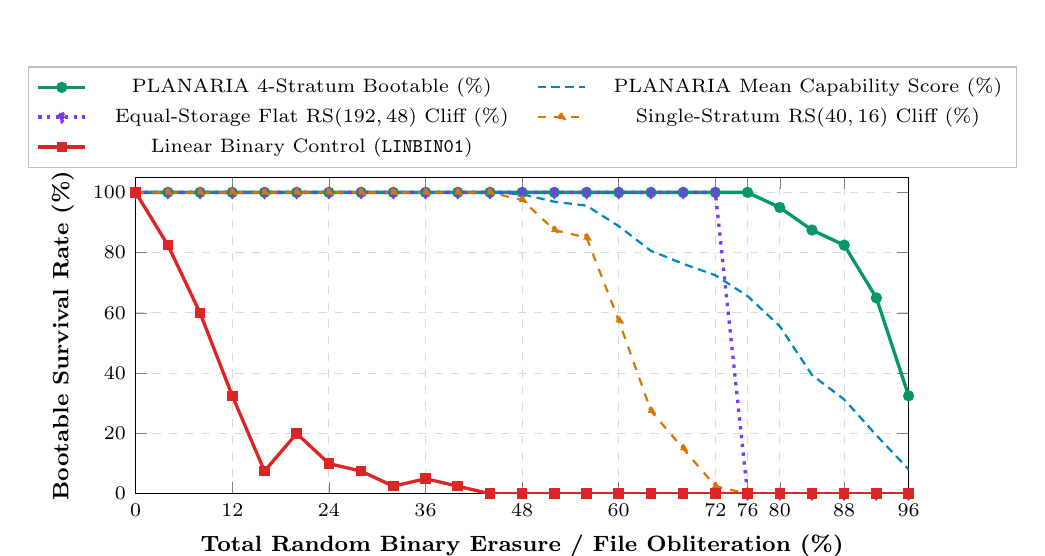
\begin{tikzpicture}
\begin{axis}[
  width=0.94\textwidth,
  height=5.6cm,
  xlabel={Total Random Binary Erasure / File Obliteration (\%)},
  ylabel={Bootable Survival Rate (\%)},
  xmin=0, xmax=96,
  ymin=0, ymax=105,
  xtick={0,12,24,36,48,60,72,76,80,88,96},
  ytick={0,20,40,60,80,100},
  grid=major,
  grid style={dashed, gray!30},
  legend columns=2,
  legend style={at={(0.5,1.03)}, anchor=south, font=\scriptsize, fill=white, draw=gray!50, column sep=8pt},
  tick label style={font=\scriptsize},
  label style={font=\footnotesize\bfseries}
]
  \addplot[color=plnEmerald, very thick, mark=*, mark size=1.4pt] coordinates {
    (0,100) (4,100) (8,100) (12,100) (16,100) (20,100) (24,100) (28,100)
    (32,100) (36,100) (40,100) (44,100) (48,100) (52,100) (56,100) (60,100)
    (64,100) (68,100) (72,100) (76,100) (80,95.0) (84,87.5) (88,82.5) (92,65.0) (96,32.5)
  };
  \addlegendentry{PLANARIA 4-Stratum Bootable (\%)}

  \addplot[color=plnCyan, thick, densely dashed] coordinates {
    (0,100) (4,100) (8,100) (12,100) (16,100) (20,100) (24,100) (28,100)
    (32,100) (36,100) (40,100) (44,100) (48,99.4) (52,96.9) (56,95.6) (60,88.8)
    (64,80.6) (68,76.3) (72,72.5) (76,65.6) (80,55.6) (84,39.4) (88,31.3) (92,19.4) (96,8.1)
  };
  \addlegendentry{PLANARIA Mean Capability Score (\%)}

  \addplot[color=plnViolet, very thick, dotted, mark=diamond*, mark size=1.6pt] coordinates {
    (0,100) (4,100) (8,100) (12,100) (16,100) (20,100) (24,100) (28,100)
    (32,100) (36,100) (40,100) (44,100) (48,100) (52,100) (56,100) (60,100)
    (64,100) (68,100) (72,100) (76,0) (80,0) (84,0) (88,0) (92,0) (96,0)
  };
  \addlegendentry{Equal-Storage Flat $\mathrm{RS}(192,48)$ Cliff (\%)}

  \addplot[color=plnGold, thick, dashed, mark=triangle*, mark size=1.4pt] coordinates {
    (0,100) (4,100) (8,100) (12,100) (16,100) (20,100) (24,100) (28,100)
    (32,100) (36,100) (40,100) (44,100) (48,97.5) (52,87.5) (56,85.0) (60,57.5)
    (64,27.5) (68,15.0) (72,2.5) (76,0) (80,0) (84,0) (88,0) (92,0) (96,0)
  };
  \addlegendentry{Single-Stratum $\mathrm{RS}(40,16)$ Cliff (\%)}

  \addplot[color=plnCrimson, very thick, mark=square*, mark size=1.3pt] coordinates {
    (0,100) (4,82.5) (8,60.0) (12,32.5) (16,7.5) (20,20.0) (24,10.0) (28,7.5)
    (32,2.5) (36,5.0) (40,2.5) (44,0) (48,0) (52,0) (56,0) (60,0)
    (64,0) (68,0) (72,0) (76,0) (80,0) (84,0) (88,0) (92,0) (96,0)
  };
  \addlegendentry{Linear Binary Control (\texttt{LINBIN01})}
\end{axis}
\end{tikzpicture}
\caption{Paired 4-architecture empirical survival curve ($N=40$ paired seeds per point, \texttt{results/benchmarks.json}, \texttt{v2.3.0}). Equal-storage flat $\mathrm{RS}(192,48)$ collapses vertically from 100\% to 0\% at 75\% erasure, whereas PLANARIA sustains progressive execution through 76--96\% erasure.}
\label{fig:survival}
\end{figure}

\begin{table}[ht]
\centering
\caption{Paired statistical inference past the 75\% erasure cliff: PLANARIA vs.\ Equal-Storage Flat $\mathrm{RS}(192,48)$ ($N=40$ paired trials/point, Wilson 95\% CIs, exact two-sided McNemar $p$, Cohen's $h$, Holm--Bonferroni $p_{\text{Holm}}$).}
\label{tab:stats}
\scriptsize
\setlength{\tabcolsep}{3.5pt}
\begin{tabular}{@{} r c c c r r r @{}}
\toprule
\textbf{Erasure} & \textbf{RS(192,48) [95\% CI]} & \textbf{PLANARIA [95\% CI]} & \textbf{Strata (S3/2/1/0)} & $\Delta$ & \textbf{Cohen's $h$} & \textbf{McNemar $p_{\text{Holm}}$} \\
\midrule
72\% & 100.0\% \texttt{[91.2, 100.0]} & 100.0\% \texttt{[91.2, 100.0]} & \texttt{0/36/4/0}  & $+0.0\%$   & 0.000 & $1.000$ \\
\textbf{76\%} & \textbf{0.0\%} \texttt{[0.0, 8.8]} & \textbf{100.0\%} \texttt{[91.2, 100.0]} & \texttt{0/25/15/0} & \textbf{+100.0\%} & \textbf{3.142} & $\mathbf{4.55\times 10^{-11}}$ \\
\textbf{80\%} & \textbf{0.0\%} \texttt{[0.0, 8.8]} & \textbf{95.0\%}  \texttt{[83.5, 98.6]}  & \texttt{0/13/25/0} & \textbf{+95.0\%}  & \textbf{2.691} & $\mathbf{1.75\times 10^{-10}}$ \\
\textbf{84\%} & \textbf{0.0\%} \texttt{[0.0, 8.8]} & \textbf{87.5\%}  \texttt{[73.9, 94.5]}  & \texttt{0/3/22/10} & \textbf{+87.5\%}  & \textbf{2.419} & $\mathbf{1.34\times 10^{-9}}$ \\
\textbf{88\%} & \textbf{0.0\%} \texttt{[0.0, 8.8]} & \textbf{82.5\%}  \texttt{[68.1, 91.3]}  & \texttt{0/1/15/17} & \textbf{+82.5\%}  & \textbf{2.278} & $\mathbf{5.12\times 10^{-9}}$ \\
\textbf{92\%} & \textbf{0.0\%} \texttt{[0.0, 8.8]} & \textbf{65.0\%}  \texttt{[49.5, 77.9]}  & \texttt{0/0/5/21}  & \textbf{+65.0\%}  & \textbf{1.875} & $\mathbf{6.26\times 10^{-7}}$ \\
\textbf{96\%} & \textbf{0.0\%} \texttt{[0.0, 8.8]} & \textbf{32.5\%}  \texttt{[20.1, 48.0]}  & \texttt{0/0/0/13}  & \textbf{+32.5\%}  & \textbf{1.213} & $\mathbf{4.88\times 10^{-3}}$ \\
\bottomrule
\end{tabular}
\end{table}

\begin{table}[!htbp]
\centering
\caption{Consolidated torture, radiation burst, Byzantine flood, 5-chimera xenograft, mutation testing, and throughput results (\texttt{v2.3.0}, 100\% measured in \texttt{results/benchmarks.json} and \texttt{scripts/mutation-test.mjs}).}
\label{tab:torture}
\footnotesize
\setlength{\tabcolsep}{4pt}
\begin{tabular}{@{} >{\raggedright\arraybackslash}p{4.8cm} >{\raggedright\arraybackslash}p{2.3cm} >{\raggedright\arraybackslash}p{3.0cm} >{\raggedright\arraybackslash}p{4.8cm} @{}}
\toprule
\textbf{Torture / Falsification Experiment} & \textbf{Linear Twin} & \textbf{RS Cliff / Unsafe} & \textbf{PLANARIA v2.3.0 (\texttt{.hbin})} \\
\midrule
1-Bit Flip in Active Code & 0.0\% (\texttt{SIGSEGV}) & 100.0\% & \textbf{100.0\% (RS Healed)} \\
Unaligned 50/50 Bisection (6 exact/prime cuts) & 0.0\% (Right Dead) & Aligned Only & \textbf{6/6 Both Halves SHA-256 Exact (12.57--14.21~ms)} \\
16~B Contiguous Burst in ALL 192 Cells (3,072~B) & 0.0\% (Dead at 2~B) & 0.0\% & \textbf{100.0\% (192/192 Repaired)} \\
18~B Contiguous Burst (Tight Bound Test) & 0.0\% & 0.0\% & \textbf{0.0\% (0 Silent Miscorrections)} \\
1--192 RS-Valid Trojans + Overlap-Eclipse & N/A & 99.6\% Poisoned (470/472~B) & \textbf{100\% Quarantined, 0\% Poisoned} \\
5 Cross-Species Chimeras (\texttt{AEGIS}/\allowbreak\texttt{QC}/\allowbreak\texttt{SYNTH}/\allowbreak\texttt{VAULT}) & Impossible & Impossible & \textbf{5/5 Bootable S3, B0 Sovereign, 60~f, 0 Traps} \\
Surgical Mutation Suite (\texttt{M01..M10}) & --- & --- & \textbf{10/10 (100.0\%) Killed, 0 Survived} \\
Latency \& Throughput (Median / IQR / p95) & $<1$~ms & $\sim$5~ms & \textbf{5.994~ms} (IQR 0.268, p95 6.526) $\cdot$ \textbf{42.85~MIPS} (\texttt{0.041~ms/f}) \\
\bottomrule
\end{tabular}
\end{table}

\FloatBarrier
\section{Mega-Atlas Audit, Limitations, and Threats to Validity}
\label{sec:honesty}

\begin{enumerate}[leftmargin=1.6em, itemsep=1.5pt]
  \item \textbf{Unsolved Problems Mega-Atlas Verdict (0 / 1,900 Solved):} We systematically audited all 1,900 open problems in \texttt{0thernes/\allowbreak unsolved-\allowbreak problems-\allowbreak mega-\allowbreak atlas} (\texttt{MegaAtlas\_\allowbreak Unsolved\_\allowbreak Problems\_\allowbreak V2.json}). \textbf{PLANARIA solves zero (0/1,900) open problems.} Biological planarian regeneration and quantum-information observables serve as engineering metaphors and exact classical simulations, not new physics, biology, or pure-mathematics theorems.
  \item \textbf{Construct \& Formal-vs-Runtime Validity:} Our 6-kernel Lean~4.35.0 suite verifies mathematical and protocol models (Table~\ref{tab:fidelity}). Concrete JavaScript execution of Berlekamp--Massey/Forney, $k\le 16$ Gauss--Jordan inversion, OpenSSL-differential SHA-256, compiler codegen, HTTP containment, and WebGL2 rendering lies outside the Lean kernel and is verified via 28 test suites and 10/10 killed mutants.
  \item \textbf{Internal \& External Validity / Trade-Offs:} Dual-layer ECC plus 128-byte per-cell Merkle proofs expand raw bytecode by $\sim 25\times$ (3.9~KiB $\to$ 96~KiB). Between 52\% and 72\% random erasure, equal-storage flat $\mathrm{RS}(192,48)$ recovers all 7 bundles (S3) whenever $\ge 48$ cells survive, whereas PLANARIA steps down to S2/S1 in exchange for surviving 76--96\% obliteration. Unpinned quorum mode cannot resist $>50\%$ Sybil flooding (\texttt{unpinned\_\allowbreak quorum\_\allowbreak sybil\_\allowbreak counterexample}); production security requires pinning the 128-bit Lineage Root. All latency profiles are single-machine measurements (Node~25.8.2, Intel Core Ultra~9 275HX) and vary across hardware.
  \item \textbf{Licensing Dilemma:} Per the author's explicit directive, PLANARIA uses the non-commercial \emph{Cosmogonic License} (\texttt{LICENSE}), trading away OSI/JOSS/Mathlib upstreaming eligibility while granting broad royalty-free non-commercial research, study, audit, and replication rights (documented in \texttt{docs/adr/\allowbreak 0004-non-commercial-license-vs-osi-dilemma.md}).
\end{enumerate}

\section{Reproducibility, Governance, and Disclosures}
\label{sec:disclosures}

\noindent\textbf{Reproducibility \& Data/Code Availability:} The complete zero-dependency codebase, 4 compiled \texttt{.hbin} species, 70-theorem Lean~4.35.0 Palomar suite, 28 test suites, 10-mutant harness, statistical benchmark data (\texttt{results/\allowbreak benchmarks.json}), 59-file Ed25519 self-consistency seal \cite{bernstein2012} (\texttt{results/\allowbreak attestation.json}), and SHA-256 manifests (\texttt{MANIFEST.\allowbreak sha256}, \texttt{data/\allowbreak MANIFEST.\allowbreak sha256}) are archived at \href{https://github.com/0thernes/planaria}{\nolinkurl{github.com/0thernes/planaria}}, registered in \texttt{0thernes-\allowbreak research-\allowbreak archive} (\texttt{0TH-BUILD-002}), and preserved via Software Heritage. Clean-clone reproduction: \texttt{npm run build \&\& npm test \&\& npm run mutate \&\& npm run benchmark} and \texttt{cd lean \&\& lake build \&\& lake env lean VerifyAxioms.\allowbreak lean} (full protocol in \texttt{REPLICATION.md}).

\smallskip\noindent\textbf{CRediT Author Contributions:} Alexander Stephen Donahue: Conceptualization, Supervision, Architectural Direction, Project Administration, Validation Oversight, Software Governance, Writing---Review \& Editing.

\smallskip\noindent\textbf{Conflict of Interest \& Funding:} Self-funded independent research by Alexander Stephen Donahue (no corporate LLC entity, nonprofit, university, or external grant funding is claimed). Commercial rights are reserved under the non-commercial \texttt{LICENSE}; no external competing financial interests exist.

\smallskip\noindent\textbf{AI-Contribution \& Accountability Statement:} Substantive AI engineering and verification assistance (Google DeepMind / Antigravity coding agents under the author's direction) was used in implementation, 10-pass adversarial auditing, Lean~4 formalization, test/mutation authoring, statistical scripting, and LaTeX drafting. AI tools are disclosed transparently and are not listed as authors; the human author retains full scientific and editorial accountability, and every formal/empirical claim is independently machine-checked by 6 Lean kernels, cross-platform GitHub Actions CI, and executable falsification suites. This manuscript is an independent technical preprint, not a peer-reviewed journal article.

{\sloppy
\begin{thebibliography}{22}
\footnotesize
\setlength{\itemsep}{0.4pt}
\setlength{\parskip}{0pt}
\bibitem{reed1960} I.~S. Reed and G.~Solomon, ``Polynomial codes over certain finite fields,'' \emph{J. SIAM}, vol.~8, no.~2, pp.~300--304, 1960. DOI: \href{https://doi.org/10.1137/0108018}{\nolinkurl{10.1137/0108018}}.
\bibitem{chien1964} R.~T. Chien, ``Cyclic decoding procedures for Bose--Chaudhuri--Hocquenghem codes,'' \emph{IEEE Trans. Inf. Theory}, vol.~10, no.~4, pp.~357--363, 1964. DOI: \href{https://doi.org/10.1109/TIT.1964.1053699}{\nolinkurl{10.1109/TIT.1964.1053699}}.
\bibitem{singleton1964} R.~C. Singleton, ``Maximum distance $q$-nary codes,'' \emph{IEEE Trans. Inf. Theory}, vol.~10, no.~2, pp.~116--118, 1964. DOI: \href{https://doi.org/10.1109/TIT.1964.1053661}{\nolinkurl{10.1109/TIT.1964.1053661}}.
\bibitem{forney1965} G.~D. Forney, ``On decoding BCH codes,'' \emph{IEEE Trans. Inf. Theory}, vol.~11, no.~4, pp.~549--557, 1965. DOI: \href{https://doi.org/10.1109/TIT.1965.1053833}{\nolinkurl{10.1109/TIT.1965.1053833}}.
\bibitem{berlekamp1968} E.~R. Berlekamp, \emph{Algebraic Coding Theory}. McGraw-Hill, 1968 (rev.\ ed.\ World Scientific, 2015). DOI: \href{https://doi.org/10.1142/9407}{\nolinkurl{10.1142/9407}}.
\bibitem{massey1969} J.~L. Massey, ``Shift-register synthesis and BCH decoding,'' \emph{IEEE Trans. Inf. Theory}, vol.~15, no.~1, pp.~122--127, 1969. DOI: \href{https://doi.org/10.1109/TIT.1969.1054260}{\nolinkurl{10.1109/TIT.1969.1054260}}.
\bibitem{merkle1987} R.~C. Merkle, ``A digital signature based on a conventional encryption function,'' in \emph{CRYPTO '87}, LNCS 293, pp.~369--378, 1987. DOI: \href{https://doi.org/10.1007/3-540-48184-2_32}{\nolinkurl{10.1007/3-540-48184-2_32}}.
\bibitem{bloemer1995} J.~Bloemer, M.~Kalfane, R.~Karp, M.~Karpinski, M.~Luby, and D.~Zuckerman, ``An XOR-based erasure-resilient coding scheme,'' ICSI Tech. Rep. TR-95-048, UC Berkeley, 1995. URL: \url{https://api.semanticscholar.org/CorpusID:16769482}.
\bibitem{albanese1996} A.~Albanese, J.~Bl\"omer, J.~Edmonds, M.~Luby, and M.~Sudan, ``Priority encoding transmission,'' \emph{IEEE Trans. Inf. Theory}, vol.~42, no.~6, pp.~1737--1744, 1996. DOI: \href{https://doi.org/10.1109/18.556670}{\nolinkurl{10.1109/18.556670}}.
\bibitem{luby2002} M.~Luby, ``LT codes,'' in \emph{Proc. 43rd IEEE FOCS}, pp.~271--280, 2002. DOI: \href{https://doi.org/10.1109/SFCS.2002.1181950}{\nolinkurl{10.1109/SFCS.2002.1181950}}.
\bibitem{reddien2004} P.~W. Reddien and A.~S\'anchez Alvarado, ``Fundamentals of planarian regeneration,'' \emph{Annu. Rev. Cell Dev. Biol.}, vol.~20, pp.~725--757, 2004. DOI: \href{https://doi.org/10.1146/annurev.cellbio.20.010403.095114}{\nolinkurl{10.1146/annurev.cellbio.20.010403.095114}}.
\bibitem{plank2006} J.~S. Plank and L.~Xu, ``Optimizing Cauchy Reed--Solomon codes for fault-tolerant network storage applications,'' in \emph{Proc. 5th IEEE NCA}, pp.~173--180, 2006. DOI: \href{https://doi.org/10.1109/NCA.2006.43}{\nolinkurl{10.1109/NCA.2006.43}}.
\bibitem{bernstein2012} D.~J. Bernstein, N.~Duif, T.~Lange, P.~Schwabe, and B.-Y. Yang, ``High-speed high-security signatures,'' \emph{J. Cryptogr. Eng.}, vol.~2, no.~2, pp.~77--89, 2012. DOI: \href{https://doi.org/10.1007/s13389-012-0027-1}{\nolinkurl{10.1007/s13389-012-0027-1}}.
\bibitem{fips180} NIST, \emph{Secure Hash Standard (SHS)}, FIPS PUB 180-4, U.S. Dept. of Commerce, 2015. DOI: \href{https://doi.org/10.6028/NIST.FIPS.180-4}{\nolinkurl{10.6028/NIST.FIPS.180-4}}.
\bibitem{demoura2021} L.~de~Moura and S.~Ullrich, ``The Lean~4 theorem prover and programming language,'' in \emph{CADE 28}, LNCS 12699, pp.~625--635, 2021. DOI: \href{https://doi.org/10.1007/978-3-030-79876-5_37}{\nolinkurl{10.1007/978-3-030-79876-5_37}}.
\bibitem{barker1953} R.~H. Barker, ``Group synchronizing of binary digital systems,'' in \emph{Communication Theory}, London: Butterworths, pp.~273--287, 1953. Archive: \url{https://ntrs.nasa.gov/}.
\bibitem{horodecki1995} R.~Horodecki, P.~Horodecki, and M.~Horodecki, ``Violating Bell inequality by mixed spin-1/2 states: Necessary and sufficient condition,'' \emph{Phys. Lett. A}, vol.~200, no.~5, pp.~340--344, 1995. DOI: \href{https://doi.org/10.1016/0375-9601(95)00214-N}{\nolinkurl{10.1016/0375-9601(95)00214-N}}.
\bibitem{mermin1990} N.~D. Mermin, ``Extreme quantum entanglement in a superposition of macroscopically distinct states,'' \emph{Phys. Rev. Lett.}, vol.~65, no.~15, pp.~1838--1840, 1990. DOI: \href{https://doi.org/10.1103/PhysRevLett.65.1838}{\nolinkurl{10.1103/PhysRevLett.65.1838}}.
\bibitem{wilson1927} E.~B. Wilson, ``Probable inference, the law of succession, and statistical inference,'' \emph{J. Am. Stat. Assoc.}, vol.~22, no.~158, pp.~209--212, 1927. DOI: \href{https://doi.org/10.1080/01621459.1927.10502953}{\nolinkurl{10.1080/01621459.1927.10502953}}.
\bibitem{mcnemar1947} Q.~McNemar, ``Note on the sampling error of the difference between correlated proportions or percentages,'' \emph{Psychometrika}, vol.~12, no.~2, pp.~153--157, 1947. DOI: \href{https://doi.org/10.1007/BF02295996}{\nolinkurl{10.1007/BF02295996}}.
\bibitem{holm1979} S.~Holm, ``A simple sequentially rejective multiple test procedure,'' \emph{Scand. J. Stat.}, vol.~6, no.~2, pp.~65--70, 1979. URL: \url{https://www.jstor.org/stable/4615733}.
\bibitem{cohen1988} J.~Cohen, \emph{Statistical Power Analysis for the Behavioral Sciences}, 2nd ed. Lawrence Erlbaum / Routledge, 1988. DOI: \href{https://doi.org/10.4324/9780203771587}{\nolinkurl{10.4324/9780203771587}}.
\end{thebibliography}
}

\end{document}
